\documentclass[11pt]{article}
\def\figlang{en}
\usepackage[a4paper,top=2.4cm,bottom=2.4cm,left=2.3cm,right=2.3cm,headsep=0.8cm,footskip=1cm]{geometry}
% Compatible XeLaTeX / LuaLaTeX (recommandé) et pdfLaTeX
\usepackage{iftex}
\ifPDFTeX
  \usepackage[T1]{fontenc}
  \usepackage[utf8]{inputenc}
  \usepackage{textcomp}
  \IfFileExists{tgtermes.sty}{\usepackage{tgtermes}}{\usepackage{mathptmx}}
  \IfFileExists{tgheros.sty}{\usepackage{tgheros}}{\usepackage[scaled=0.92]{helvet}}
\else
  \usepackage{fontspec}
  \setmainfont{TeX Gyre Termes}
  \setsansfont{TeX Gyre Heros}
\fi
\usepackage{amsmath,amssymb}
\usepackage{graphicx,booktabs,tabularx,array,multirow,float,enumitem}
\usepackage[table]{xcolor}
% Version de soumission : texte en noir sur fond blanc
\definecolor{navy}{HTML}{000000}\definecolor{ora}{HTML}{000000}\definecolor{fond}{HTML}{FFFFFF}
\usepackage[font=small,labelfont={bf,sf,color=navy},labelsep=period,justification=justified,singlelinecheck=false]{caption}
\captionsetup[table]{position=top,skip=4pt}
\usepackage{titlesec}
\titleformat{\section}{\sffamily\large\bfseries\color{navy}}{\thesection.}{0.5em}{}
\titleformat{\subsection}{\sffamily\normalsize\bfseries\color{navy}}{\thesubsection.}{0.5em}{}
\titleformat{\subsubsection}{\sffamily\normalsize\itshape\color{navy}}{\thesubsubsection.}{0.5em}{}
\titlespacing*{\section}{0pt}{14pt}{6pt}\titlespacing*{\subsection}{0pt}{10pt}{4pt}\titlespacing*{\subsubsection}{0pt}{8pt}{3pt}
\usepackage{fancyhdr}\pagestyle{fancy}\fancyhf{}
\renewcommand{\headrulewidth}{0.4pt}
\usepackage{tcolorbox}
\usepackage[hidelinks]{hyperref}
\usepackage{microtype}
\setlength{\parskip}{2pt}\setlength{\emergencystretch}{2em}\setlength{\parindent}{1.2em}
\linespread{1.06}
\setlist{itemsep=1pt,topsep=3pt,leftmargin=1.6em}
\renewcommand{\arraystretch}{1.15}
\newcommand{\fig}[3]{\begin{figure}[!htbp]\centering\includegraphics[width=#2\linewidth]{figures/\figlang_#1.png}\caption{#3}\label{fig:#1}\end{figure}}
\newcolumntype{R}{>{\raggedleft\arraybackslash}X}
\newcolumntype{L}{>{\raggedright\arraybackslash}X}

\ifPDFTeX\usepackage[english]{babel}\else\usepackage{polyglossia}\setmainlanguage{english}\fi
\usepackage{rotating}
\hypersetup{colorlinks=true,linkcolor=black,urlcolor=black,citecolor=black}
\fancyhead[L]{\sffamily\footnotesize\color{navy} Rainfall and typhoid fever in the Far North Region of Cameroon}
\fancyhead[R]{\sffamily\footnotesize\color{navy} Kazoune Bouba et al.}
\fancyfoot[C]{\sffamily\footnotesize\thepage}
\begin{document}\sloppy
\thispagestyle{fancy}
\noindent{\sffamily\footnotesize\color{ora}\textbf{RESEARCH ARTICLE}\hfill\color{navy} Open Access}\par\vspace{2pt}
\noindent{\color{navy}\rule{\linewidth}{1.2pt}}\par\vspace{8pt}
{\raggedright\sffamily\bfseries\LARGE\color{navy}Influence of rainfall on the dynamics and forecasting of typhoid fever in the Far North Region of Cameroon\par}
\vspace{10pt}
\noindent{\sffamily\normalsize Kazoune Bouba Israel\textsuperscript{1,2,*}, Maïrousgou Céline\textsuperscript{1}, Kidwang Jean Pierre\textsuperscript{1}, Kolaye Guilsou Gabriel\textsuperscript{2,*}\par}
\vspace{4pt}
\noindent{\footnotesize\textsuperscript{1}\,Regional Delegation of Public Health of the Far North, Maroua, Cameroon\\
\textsuperscript{2}\,National Advanced School of Engineering of Maroua, University of Maroua, Maroua, Cameroon\\
\textsuperscript{*}\,Corresponding authors: \href{mailto:kazouneisraelbouba@gmail.com}{kazouneisraelbouba@gmail.com}; \href{mailto:kolayegg@gmail.com}{kolayegg@gmail.com}\par}
\vspace{10pt}
\begin{tcolorbox}[colback=white,colframe=black,boxrule=0.5pt,arc=0pt,left=8pt,right=8pt,top=6pt,bottom=6pt,fontupper=\small]
{\sffamily\bfseries\color{navy}Abstract}\par\vspace{3pt}
\textbf{Background.} Typhoid fever is a major health burden in the Far North Region of Cameroon, characterised by a single rainy season: more than 400,000 cases were reported there between 2019 and 2025. We studied the influence of rainfall on its dynamics and assessed whether rainfall helps forecast cases, in order to guide health district preparedness.\par
\textbf{Methods.} We analysed 417,910 cases reported to DHIS2 by 522 health facilities in 32 districts (2019–2025), combined with satellite rainfall data. A transmission model with an environmental reservoir, in which rainfall contaminates water, was used to formulate hypotheses. The rainfall–case relationship was measured after detrending, distinguishing the timing of the season from its intensity. Several forecasting methods, with and without rainfall, were evaluated over three years (2023–2025) and compared with the Diebold–Mariano test.\par
\textbf{Results.} Cases peaked in October, about two months after the August rainfall peak (maximum correlation 0.54 at 8 weeks). In contrast, a wetter-than-normal season did not lead to more cases, and adding rainfall did not improve forecasts. A machine learning model shared across the 32 districts reduced four-week forecast error by 15\% relative to the benchmark method ($p<0.001$). The rise in cases between 2019 and 2022 coincided with a tripling of the number of reporting facilities.\par
\textbf{Conclusion.} Rainfall sets the timing of the typhoid season but not its intensity: district preparedness can be planned from July, while reducing peaks depends on water, sanitation and diagnosis.\par\vspace{3pt}
\textbf{Keywords:} typhoid fever; rainfall; seasonality; mathematical modelling; forecasting; surveillance; DHIS2; Far North; Cameroon
\end{tcolorbox}

\begin{tcolorbox}[colback=white,colframe=black,boxrule=0.5pt,arc=0pt,left=8pt,right=8pt,top=5pt,bottom=5pt,fontupper=\small]
{\sffamily\bfseries\color{ora}Key messages}\par\vspace{2pt}
\textbf{What was already known.} Typhoid is transmitted through contaminated water and increases during the rainy season in several countries; African data remain scarce.\par
\textbf{What this study adds.} In the Far North Region of Cameroon, the typhoid peak occurs about two months after the rainfall peak, consistently over seven years; rainfall tells \textit{when} the season will come, not \textit{how many} cases there will be. A single model for all 32 districts forecasts cases one month ahead better than conventional methods.\par
\textbf{Implications for practice.} Prepare districts from July; prioritise districts where the link with rainfall is strongest; strengthen reporting in districts with incomplete data; do not interpret rising DHIS2 case counts without accounting for network expansion.
\end{tcolorbox}

\section{Introduction}
Typhoid fever, caused by \textit{Salmonella enterica} serovar Typhi, is transmitted through water and food contaminated with faeces. It causes several million cases and more than 100,000 deaths each year, mainly in South Asia and sub-Saharan Africa [\hyperlink{ref1}{1},\hyperlink{ref2}{2}]. In sub-Saharan Africa its burden remains poorly measured, as diagnosis often relies on clinical signs or the poorly specific Widal test [\hyperlink{ref3}{3}].

In the Far North Region of Cameroon, characterised by a single rainy season, typhoid is among the most frequently reported diseases in the weekly DHIS2 surveillance system [\hyperlink{ref4}{4}]. Rainfall is likely to play a central role: it causes runoff, overflowing latrines and contamination of wells and ponds, the main water sources of many households. Understanding how rainfall influences typhoid, and whether it helps anticipate cases, would directly help district teams plan their response.

Two complementary approaches can be used to study this influence. Mathematical transmission models describe mechanisms, including the accumulation of bacteria in the environment [\hyperlink{ref5}{5},\hyperlink{ref6}{6}], but their parameters are rarely known locally. Statistical and machine learning methods learn directly from observed data and have been used to forecast typhoid in India, in several high-income countries and in Nepal, where it was associated with rainfall and flooding [\hyperlink{ref7}{7}--\hyperlink{ref9}{9}]. However, these studies rarely concern Africa, and their model comparisons often rely on a single test period, without a simple benchmark or statistical test [\hyperlink{ref10}{10}].

This study links these two approaches. Starting from a transmission model in which rainfall contaminates water, we address three questions: (i) does the typhoid season follow the rainy season, and with what lag? (ii) does a wetter-than-normal season lead to more cases? (iii) does rainfall improve case forecasts, and which forecasting method is best suited to the district level?

\section{Materials and Methods}
\subsection{Study area}
The study was conducted in the Far North Region of Cameroon, the country's northernmost region, located between 10° and 13° North latitude and 13° and 16° East longitude (Figure~\ref{fig:f2a_reference}). Covering approximately 34,263 km², it borders Nigeria to the west and Chad to the east, and reaches Lake Chad to the north. It was organised into 32 health districts over the study period, distributed among its six departments: Diamaré (Bogo, Gazawa, Maroua 1, Maroua 2, Maroua 3, Meri, Pette), Logone-et-Chari (Fotokol, Goulfey, Kousseri, Mada, Makary), Mayo-Danay (Guere, Kar-Hay, Maga, Vele, Yagoua), Mayo-Kani (Guidiguis, Kaele, Mindif, Moulvoudaye, Moutourwa), Mayo-Sava (Kolofata, Mora, Tokombere) and Mayo-Tsanaga (Bourha, Hina, Koza, Mogode, Mokolo, Mozogo, Roua).

The region has a semi-arid tropical climate, with a long dry season from October to May and a short but intense rainy season from June to September. A large part of the population obtains water from wells, boreholes and ponds, which are exposed to runoff during the rainy season. The region is also affected by insecurity linked to armed groups and by population displacement, which weaken access to care and reporting regularity in some border districts. These characteristics make the Far North a particularly relevant setting to study the link between rainfall and waterborne diseases.

\begin{sidewaysfigure}[p]\centering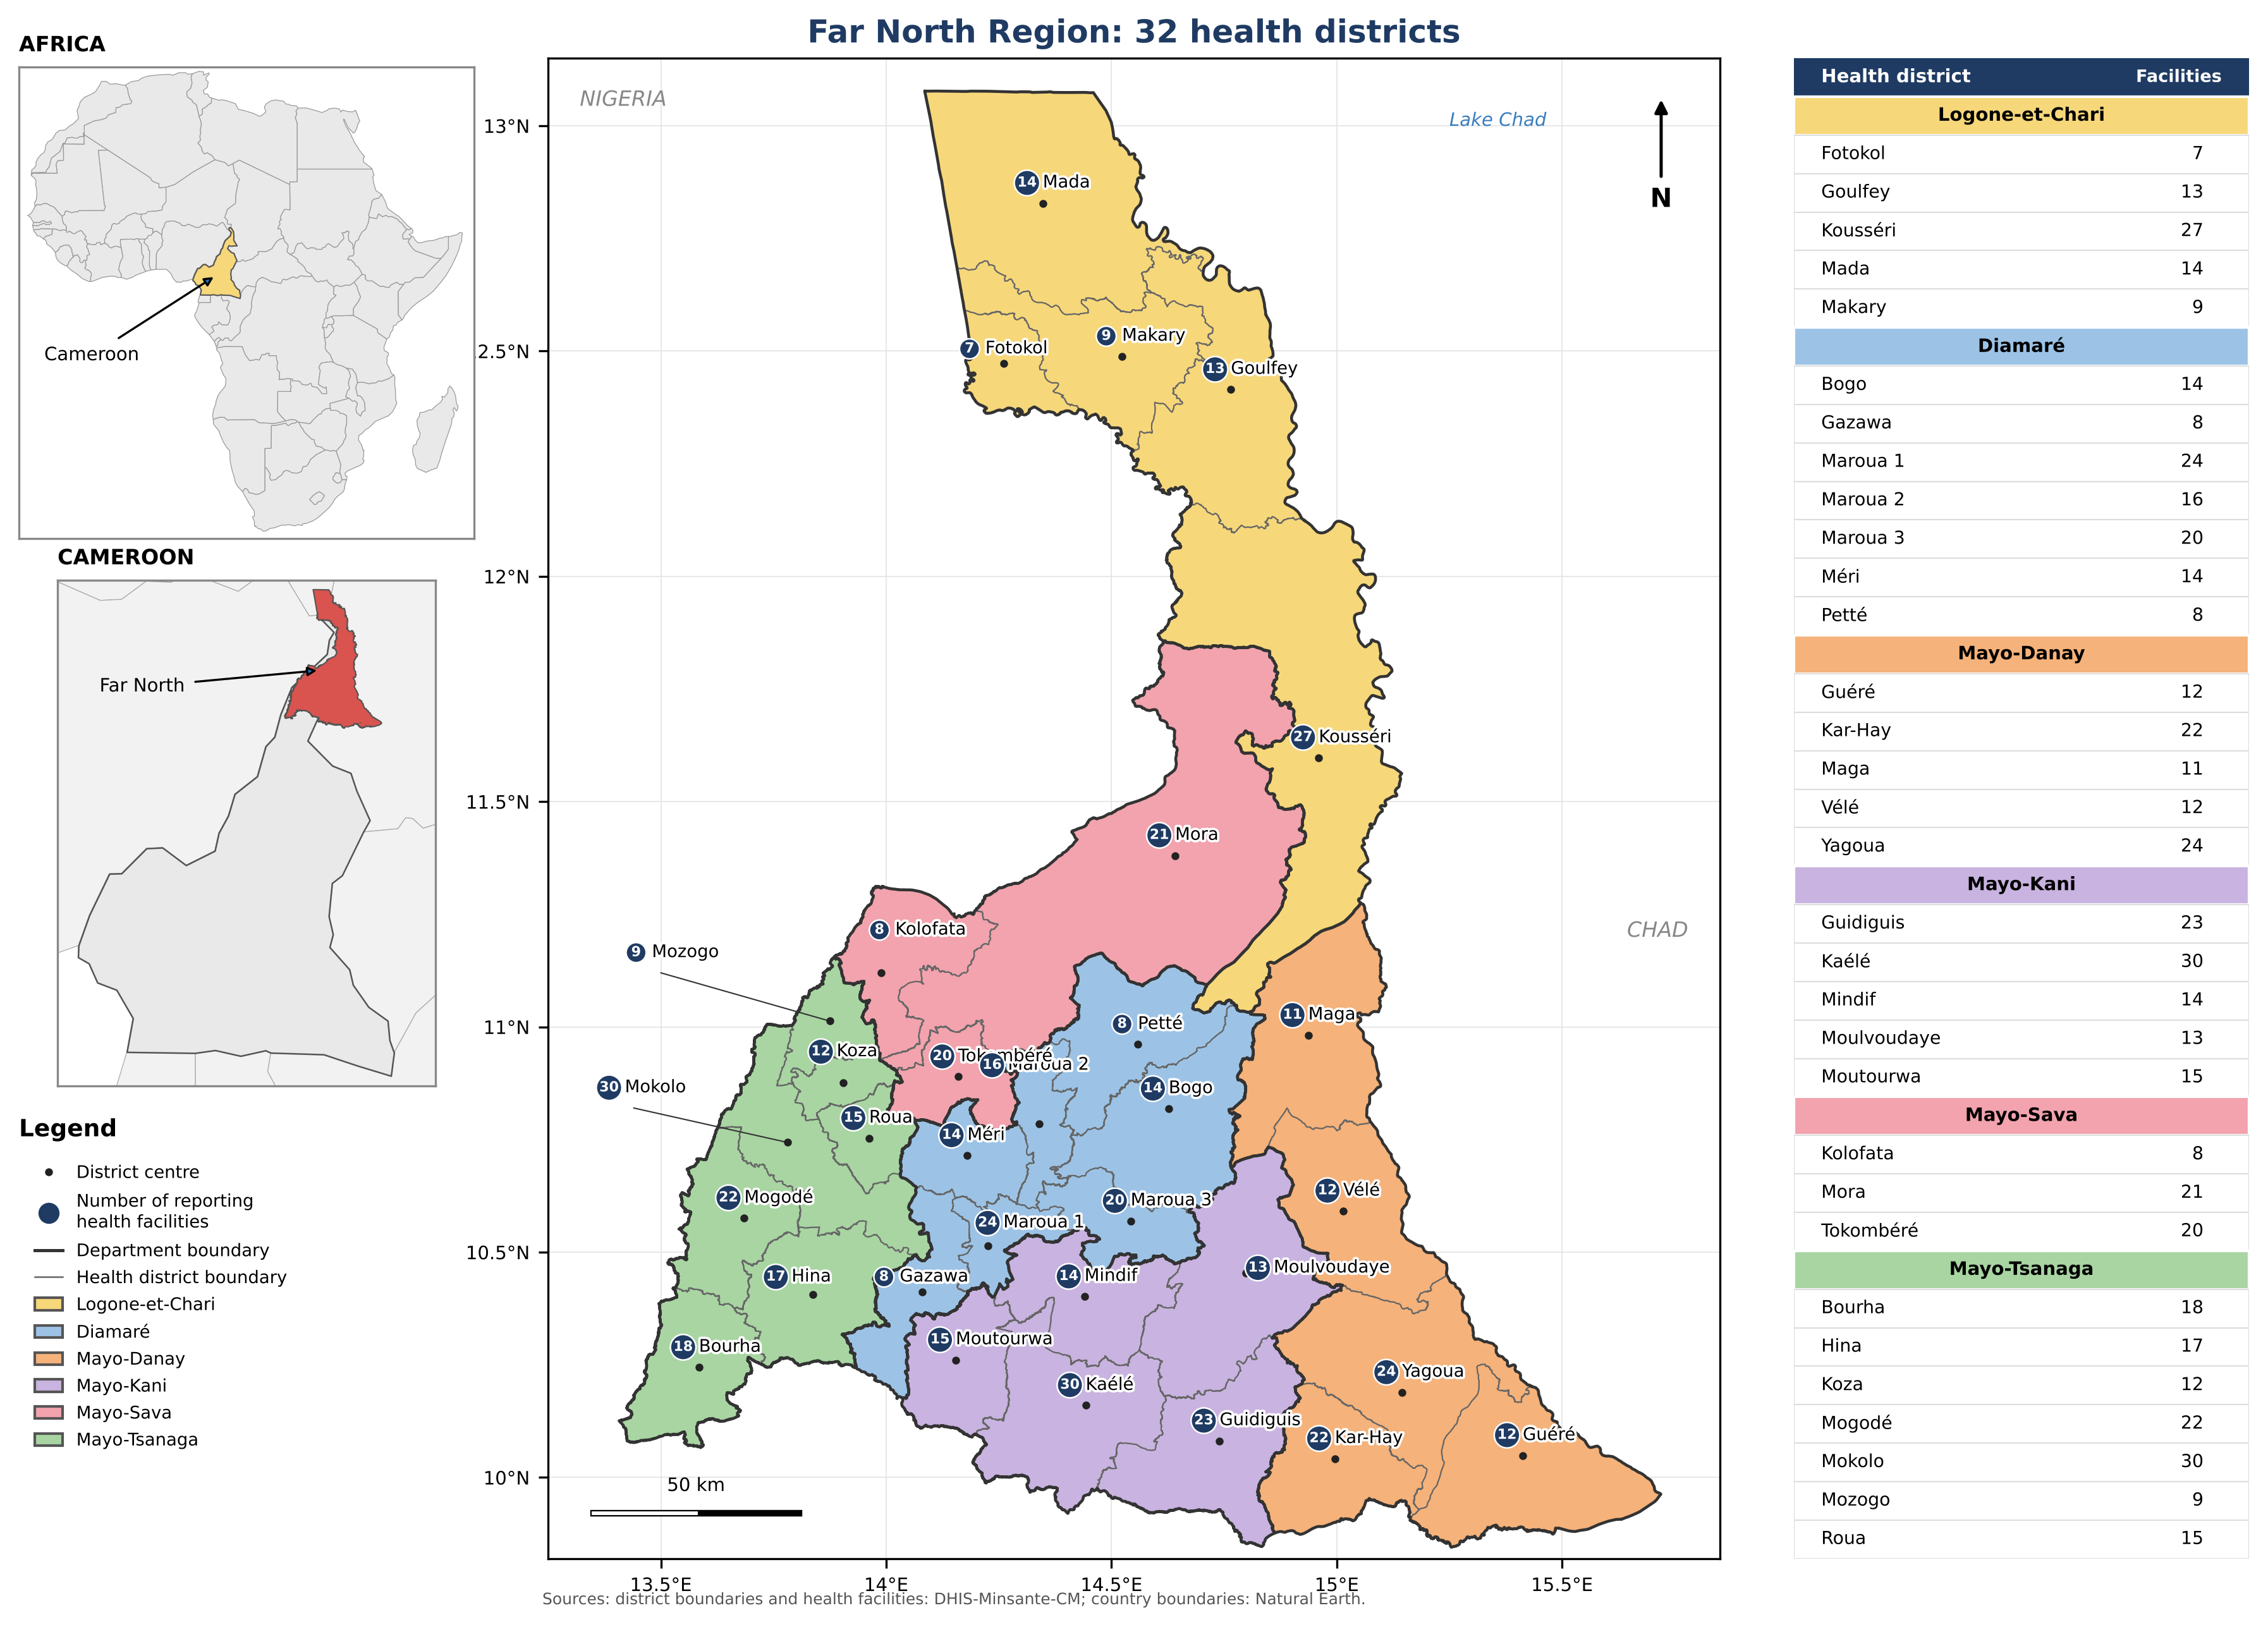
\includegraphics[width=0.95\textheight]{figures/en_zone_etude.png}\caption{Study area. Left: location of Cameroon in Africa and of the Far North Region in Cameroon, and legend. Centre: the 32 health districts, coloured by department; the number in the circle is the number of reporting health facilities in the district. Right: list of districts by department. District boundaries and health facilities: DHIS-Minsante-CM; country boundaries: Natural Earth.}\label{fig:f2a_reference}\end{sidewaysfigure}

\subsection{Data sources}
Surveillance data were extracted from DHIS-Minsante-CM (\url{https://dhis-minsante-cm.org}), the national health information system of the Ministry of Public Health, built on the DHIS2 platform [\hyperlink{ref4}{4}]. This system centralises weekly cases of diseases under surveillance reported by health facilities. Weekly typhoid cases (data element MAPE16\_H\_10) were exported for the 522 health facilities of the region, from week 1 of 2019 to week 52 of 2025 (365 weeks), in collaboration with the Regional Delegation of Public Health of the Far North. In line with national routine protocols, and in the absence of blood culture in peripheral health facilities, these cases mainly correspond to clinically suspected cases confirmed by the Widal serological test [\hyperlink{ref3}{3}]. District boundaries and the health facility hierarchy were exported from the same system.

Daily corrected precipitation, mean 2-m temperature and relative humidity were obtained from NASA POWER [\hyperlink{ref11}{11}] for one point inside each district, computed from district boundaries.

\subsection{Data pre-processing}
Pre-processing followed nine steps (Table~\ref{tab:pretraitement}). Cases exported by facility, week and age–sex category were summed by district and week, then harmonised: recently created districts were merged back into their district of origin, and the two facilities now attached to Waza were reassigned to Mora, as confirmed by historical data (250 identical weeks out of 261). The export was validated against an earlier extraction covering 2019–2023 (median difference 0\%).

A district-week without any report was considered missing and imputed by linear interpolation within the district. Unusual values were screened with the Hampel filter [\hyperlink{ref12}{12}]; as data-entry errors could not be distinguished from genuine outbreaks, they were retained. The mean–variance relationship of district cases, estimated with Taylor's power law [\hyperlink{ref13}{13}], justified the log scale used in the global model. Finally, the regional series was decomposed into trend, season and remainder with STL [\hyperlink{ref14}{14}], its stationarity assessed with the augmented Dickey–Fuller [\hyperlink{ref15}{15}] and KPSS [\hyperlink{ref16}{16}] tests, and its autocorrelation with the Ljung–Box statistic [\hyperlink{ref17}{17}]. Daily climate data were aggregated into Monday-to-Sunday weeks aligned with epidemiological weeks. The formulas for each step are given in Supplementary Material S1.

\begin{table}[!htbp]\centering\small
\caption{Data pre-processing steps.}\label{tab:pretraitement}
\begin{tabularx}{\linewidth}{@{}c >{\raggedright\arraybackslash}p{2.5cm} L >{\raggedright\arraybackslash}p{4.2cm}@{}}\toprule
No. & Step & Operation & Result \\\midrule
1 & Extraction & Raw DHIS2 export by facility, week, age and sex & 617,481 rows; 522 facilities \\
2 & Aggregation & Sum by district and week, using the hierarchy & 32 series of 365 weeks \\
3 & Harmonisation & Recently created districts merged back (Waza into Mora) & Constant boundaries over 2019–2025 \\
4 & Validation & Comparison with an earlier extraction (2019–2023) & Median difference 0\% \\
5 & Missing data & Linear interpolation within each district & 5.5\% of district-weeks imputed \\
6 & Outliers & Hampel filter (9-week window, threshold of 3 deviations) & 417 values flagged (3.8\%), retained \\
7 & Climate & Weekly aggregation of NASA POWER data & Rainfall, temperature, humidity aligned \\
8 & Transformation & $\ln(1+y)$ for the global model (Taylor's law) & Variance stabilised across districts \\
9 & Exploration & STL, ADF, KPSS, ACF/PACF, Ljung–Box & First-order differencing retained \\\bottomrule
\end{tabularx}
\end{table}

\subsection{Feature engineering}
Predictors were built using only information available at the forecast date (Table~\ref{tab:variables}). They describe recent cases, time of year and, for climate models, rainfall, temperature and humidity of previous weeks. The global model additionally receives the usual level of each district.

\begin{table}[!htbp]\centering\small
\caption{Predictors used by the XGBoost models, with rationale.}\label{tab:variables}
\begin{tabularx}{\linewidth}{@{}>{\raggedright\arraybackslash}p{4.4cm} L L@{}}\toprule
Variable & Description & Rationale \\\midrule
Cases in weeks $t$ to $t-3$ & Cases reported in the current and three previous weeks & Week-to-week persistence of cases \\
4-week mean & Mean cases over the last 4 weeks & Short-term trend, smooths noise \\
13-week mean & Mean cases over the last 13 weeks & Quarterly trend \\
Week of year (sine, cosine) & Position of the target week in the year & Seasonality; week 52 is next to week 1 \\
Same week of previous year & Cases of the target week one year earlier & Memory of the previous season \\
District level (global model) & Past mean of $\ln(1+y)$ in the district & Adapts the shared model to district size \\
4-week rainfall & Rainfall in weeks $t$ to $t-3$ & Recent rainfall effect \\
4-week rainfall lagged by 4 weeks & Rainfall in weeks $t-4$ to $t-7$ & Delayed rainfall effect (water contamination) \\
4-week temperature and humidity & Means over the last 4 weeks & Conditions for bacterial survival \\\bottomrule
\end{tabularx}
\par\smallskip\footnotesize\raggedright Climate variables are used only by the ``XGBoost with climate'' model.
\end{table}

\subsection{Study steps}
Figure~\ref{fig:pipeline2} summarises the steps followed, grouped into five phases. Surveillance, climate and boundary data were first collected (phase 1), then aggregated, checked and transformed (phase 2). The series was then explored, the mathematical model was used to formulate hypotheses, and predictors were built (phase 3). Forecasting methods were evaluated with a rolling origin and compared statistically (phase 4), before the results were translated into recommendations (phase 5).

\begin{figure}[!htbp]\centering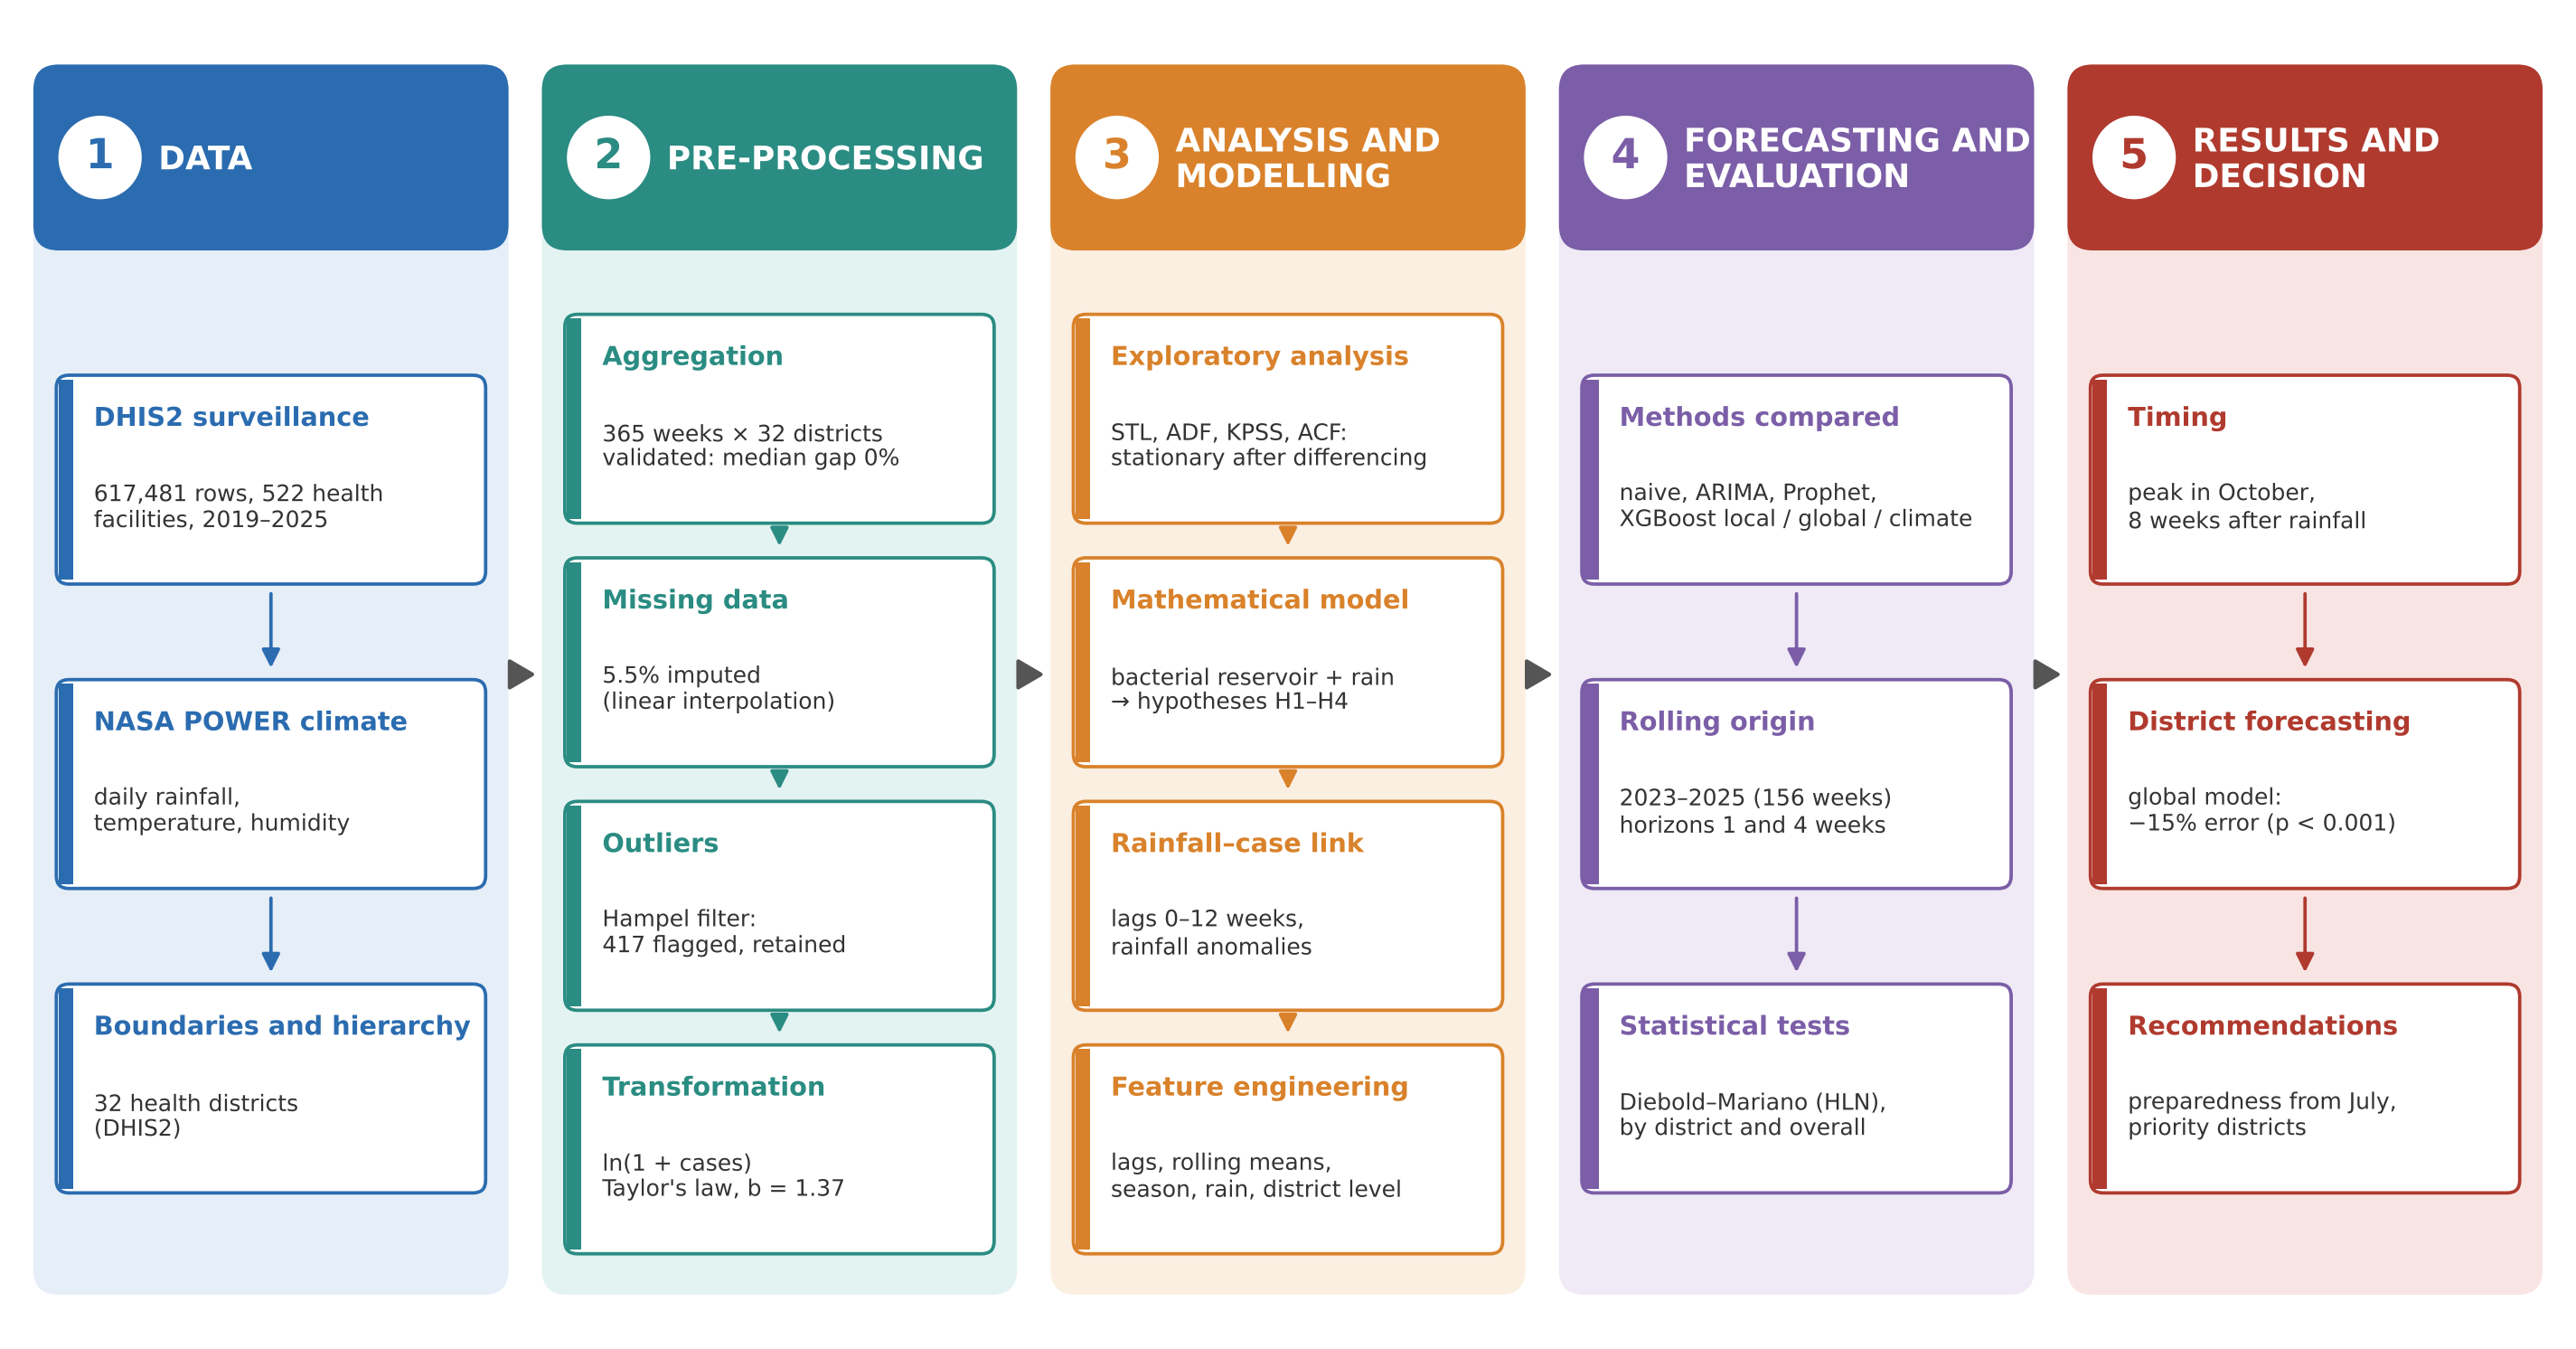
\includegraphics[width=\linewidth]{figures/en_etapes.png}\caption{Steps followed in the study, from data collection to decision support.}\label{fig:pipeline2}\end{figure}

\subsection{Mathematical modelling framework}
We started from a typhoid transmission model with an environmental reservoir [\hyperlink{ref5}{5},\hyperlink{ref6}{6}] (Figure~\ref{fig:schema_modele}). The population is divided into susceptible individuals, asymptomatic carriers, infected and recovered individuals; carriers and infected individuals shed bacteria that accumulate in water and food. The infection risk of a susceptible person, or force of infection $\lambda$, depends on the bacterial concentration $B$ through a saturating function:
\begin{equation}
\lambda(t)=\frac{\nu\,B(t)}{K+B(t)} ,
\label{eq:lambda}
\end{equation}
where $\nu$ is the maximum risk and $K$ the concentration at which the risk reaches half its maximum. We added the effect of rainfall $P(t)$, which increases environmental contamination with intensity $\kappa$, while bacteria decay at rate $\mu_b$:
\begin{equation}
\frac{dB}{dt}=\sigma_1 C+\sigma_2 I+\kappa\,P(t)-\mu_b B ,
\label{eq:pluie}
\end{equation}
where $C$ and $I$ are carriers and infected individuals, and $\sigma_1$, $\sigma_2$ their shedding rates.

\fig{schema_modele}{0.85}{Typhoid fever transmission model with an environmental reservoir and the effect of rainfall. S: susceptible; C: carriers; I: infected; R: recovered; B: bacteria in water and food. Parameters are defined in Supplementary Material S1.}

This model leads to two testable predictions. First, rainfall does not act immediately: it must first contaminate the reservoir, then the infection must incubate (about 6–30 days [\hyperlink{ref6}{6}]) before consultation and reporting; the case peak should therefore follow the rainfall peak by several weeks. Second, function~\eqref{eq:lambda} saturates: when the environment is already highly contaminated, extra rainfall hardly increases risk; a wetter-than-normal season might then not produce more cases. As the parameters are not known for the Far North, the model was not fitted: it was used to formulate these hypotheses, which were tested on the data.

\subsection{Rainfall–case relationship}
To separate seasonality from the trend linked to network expansion, each week's cases were divided by their mean over the surrounding 52 weeks. These detrended cases were correlated with rainfall accumulated over the previous 4 weeks, for lags of 0 to 12 weeks. To distinguish timing from intensity, the analysis was repeated with the rainfall anomaly, i.e. the deviation from the usual rainfall of the same week of the year. Monthly seasonal indices were also computed, following an approach similar to Shashvat et al. [\hyperlink{ref7}{7}]. Analyses were conducted for the region and for each district; associations between district characteristics were tested with Spearman correlation.

\subsection{Case forecasting and evaluation}
We compared the so-called ``naive'' benchmark, which carries forward the current week's value; the same week of the previous year; the statistical model ARIMA [\hyperlink{ref18}{18}]; Prophet [\hyperlink{ref19}{19}]; and XGBoost [\hyperlink{ref20}{20}], with and without climate variables (Table~\ref{tab:hyper}). At district level, we compared district-specific models with a single model trained on all 32 districts at once, called the global model [\hyperlink{ref21}{21},\hyperlink{ref22}{22}]. This model predicts the relative change in cases of each district $d$ at a horizon of $h$ weeks:
\begin{equation}
\ln(1+y_{d,t+h})-\ln(1+y_{d,t})=F_h\big(\mathbf{x}_{d,t},\,\bar{u}_{d,t}\big)+\varepsilon_{d,t+h} ,
\label{eq:global}
\end{equation}
where $y_{d,t}$ is the number of cases, $\mathbf{x}_{d,t}$ the predictors of Table~\ref{tab:variables}, $\bar{u}_{d,t}$ the usual level of the district, and $F_h$ a single function learned from all districts.

\begin{table}[!htbp]\centering\small
\caption{Specification of the forecasting methods.}\label{tab:hyper}
\begin{tabularx}{\linewidth}{@{}>{\raggedright\arraybackslash}p{3.6cm} L L@{}}\toprule
Method & Specification & Parameters \\\midrule
Naive; same week of previous year & Carry forward the last value; value one year earlier & None \\
ARIMA & Order chosen on 2019–2022 (KPSS, Akaike criterion), then fixed & Regional: ARIMA(2,1,1); one order per district \\
Prophet & Piecewise trend and annual seasonality & Fourier series of order 10 \\
XGBoost (local, global, with climate) & One model per horizon; forecasts the change in cases & 300 trees; depth 3; learning rate 0.05; subsampling 0.8 \\\bottomrule
\end{tabularx}
\par\smallskip\footnotesize\raggedright Settings were fixed before evaluation and never tuned on the test period.
\end{table}

One- and four-week-ahead forecasts were evaluated over 2023–2025 (156 weeks), when the surveillance network was stable. Each week, each model was retrained on past data only, as in real conditions (rolling origin [\hyperlink{ref23}{23}]). Accuracy was measured by the mean absolute error (MAE) [\hyperlink{ref24}{24}], root mean squared error (RMSE) and percentage error (MAPE). Differences between methods were tested with the Diebold–Mariano test [\hyperlink{ref25}{25}] with the Harvey–Leybourne–Newbold correction [\hyperlink{ref26}{26}], district by district and across all districts. The regional evaluation was repeated excluding districts with incomplete data.

\subsection{Software and ethics}
Analyses were performed in Python (pandas, statsmodels, prophet, xgboost, scipy); analysis scripts are deposited in a public GitHub repository (\url{https://github.com/israel-12/typhoide-extreme-nord}). The study uses only aggregated routine surveillance data, without individual information; their use was authorised by the Regional Delegation of Public Health of the Far North (DRSP-EN).

\section{Results}
\subsection{Data description}
Between 2019 and 2025, 417,910 cases were reported, an average of 1,145 per week (Table~\ref{tab:desc}, Figure~\ref{fig:f3_serie}). Cases were concentrated in urban and border districts: Kousseri (13.9\%), Maroua 1 (11.0\%), Mokolo (10.0\%), Mora (5.7\%) and Yagoua (5.4\%) (Figure~\ref{fig:cartes}A). The rise in reported cases between 2019 and 2022 coincided with network expansion: the number of reporting facilities tripled, then stabilised around 360 (Table~\ref{tab:fac}). Over the stable period 2022–2025, cases increased by only 20\%.

\begin{table}[!htbp]\centering\small
\caption{Descriptive statistics of weekly reported cases, Far North Region, 2019–2025.}\label{tab:desc}
\begin{tabularx}{\linewidth}{@{}L r@{}}\toprule
Indicator & Value \\\midrule
Weeks × districts & 365 × 32 \\
Total reported cases & 417,910 \\
Cases per week (region): mean (SD) & 1,145 (315) \\
Cases per week (region): median [Q1; Q3] & 1,143 [969; 1,340] \\
Cases per week (region): minimum; maximum & 328 (June 2019); 1,956 (Sept. 2025) \\
Mean weekly cases per district: median [min; max] & 29.3 [2.2; 159.7] \\
Missing district-weeks & 5.5\% \\
Flagged outliers (Hampel filter) & 417 (3.8\%) \\\bottomrule
\end{tabularx}
\end{table}

\begin{table}[!htbp]\centering\small
\caption{Reporting health facilities, mean weekly cases and annual rainfall, Far North Region.}\label{tab:fac}
\begin{tabular}{@{}lrrrrrrr@{}}\toprule
 & 2019 & 2020 & 2021 & 2022 & 2023 & 2024 & 2025 \\\midrule
Reporting facilities (mean/week) & 104 & 145 & 231 & 334 & 358 & 359 & 364 \\
Cases per week (regional mean) & 689 & 950 & 1,147 & 1,188 & 1,258 & 1,371 & 1,425 \\
Missing district-weeks (\%) & 20.3 & 11.2 & 3.4 & 0.0 & 1.1 & 0.9 & 1.1 \\
Annual rainfall (mm, regional mean) & 829 & 627 & 545 & 822 & 623 & 832 & 748 \\\bottomrule
\end{tabular}
\end{table}

\fig{f3_serie}{0.95}{Weekly typhoid cases reported in the Far North Region (solid line) and number of reporting health facilities (dashed line), 2019–2025. The shaded area shows the forecast evaluation period.}

\begin{figure}[!htbp]\centering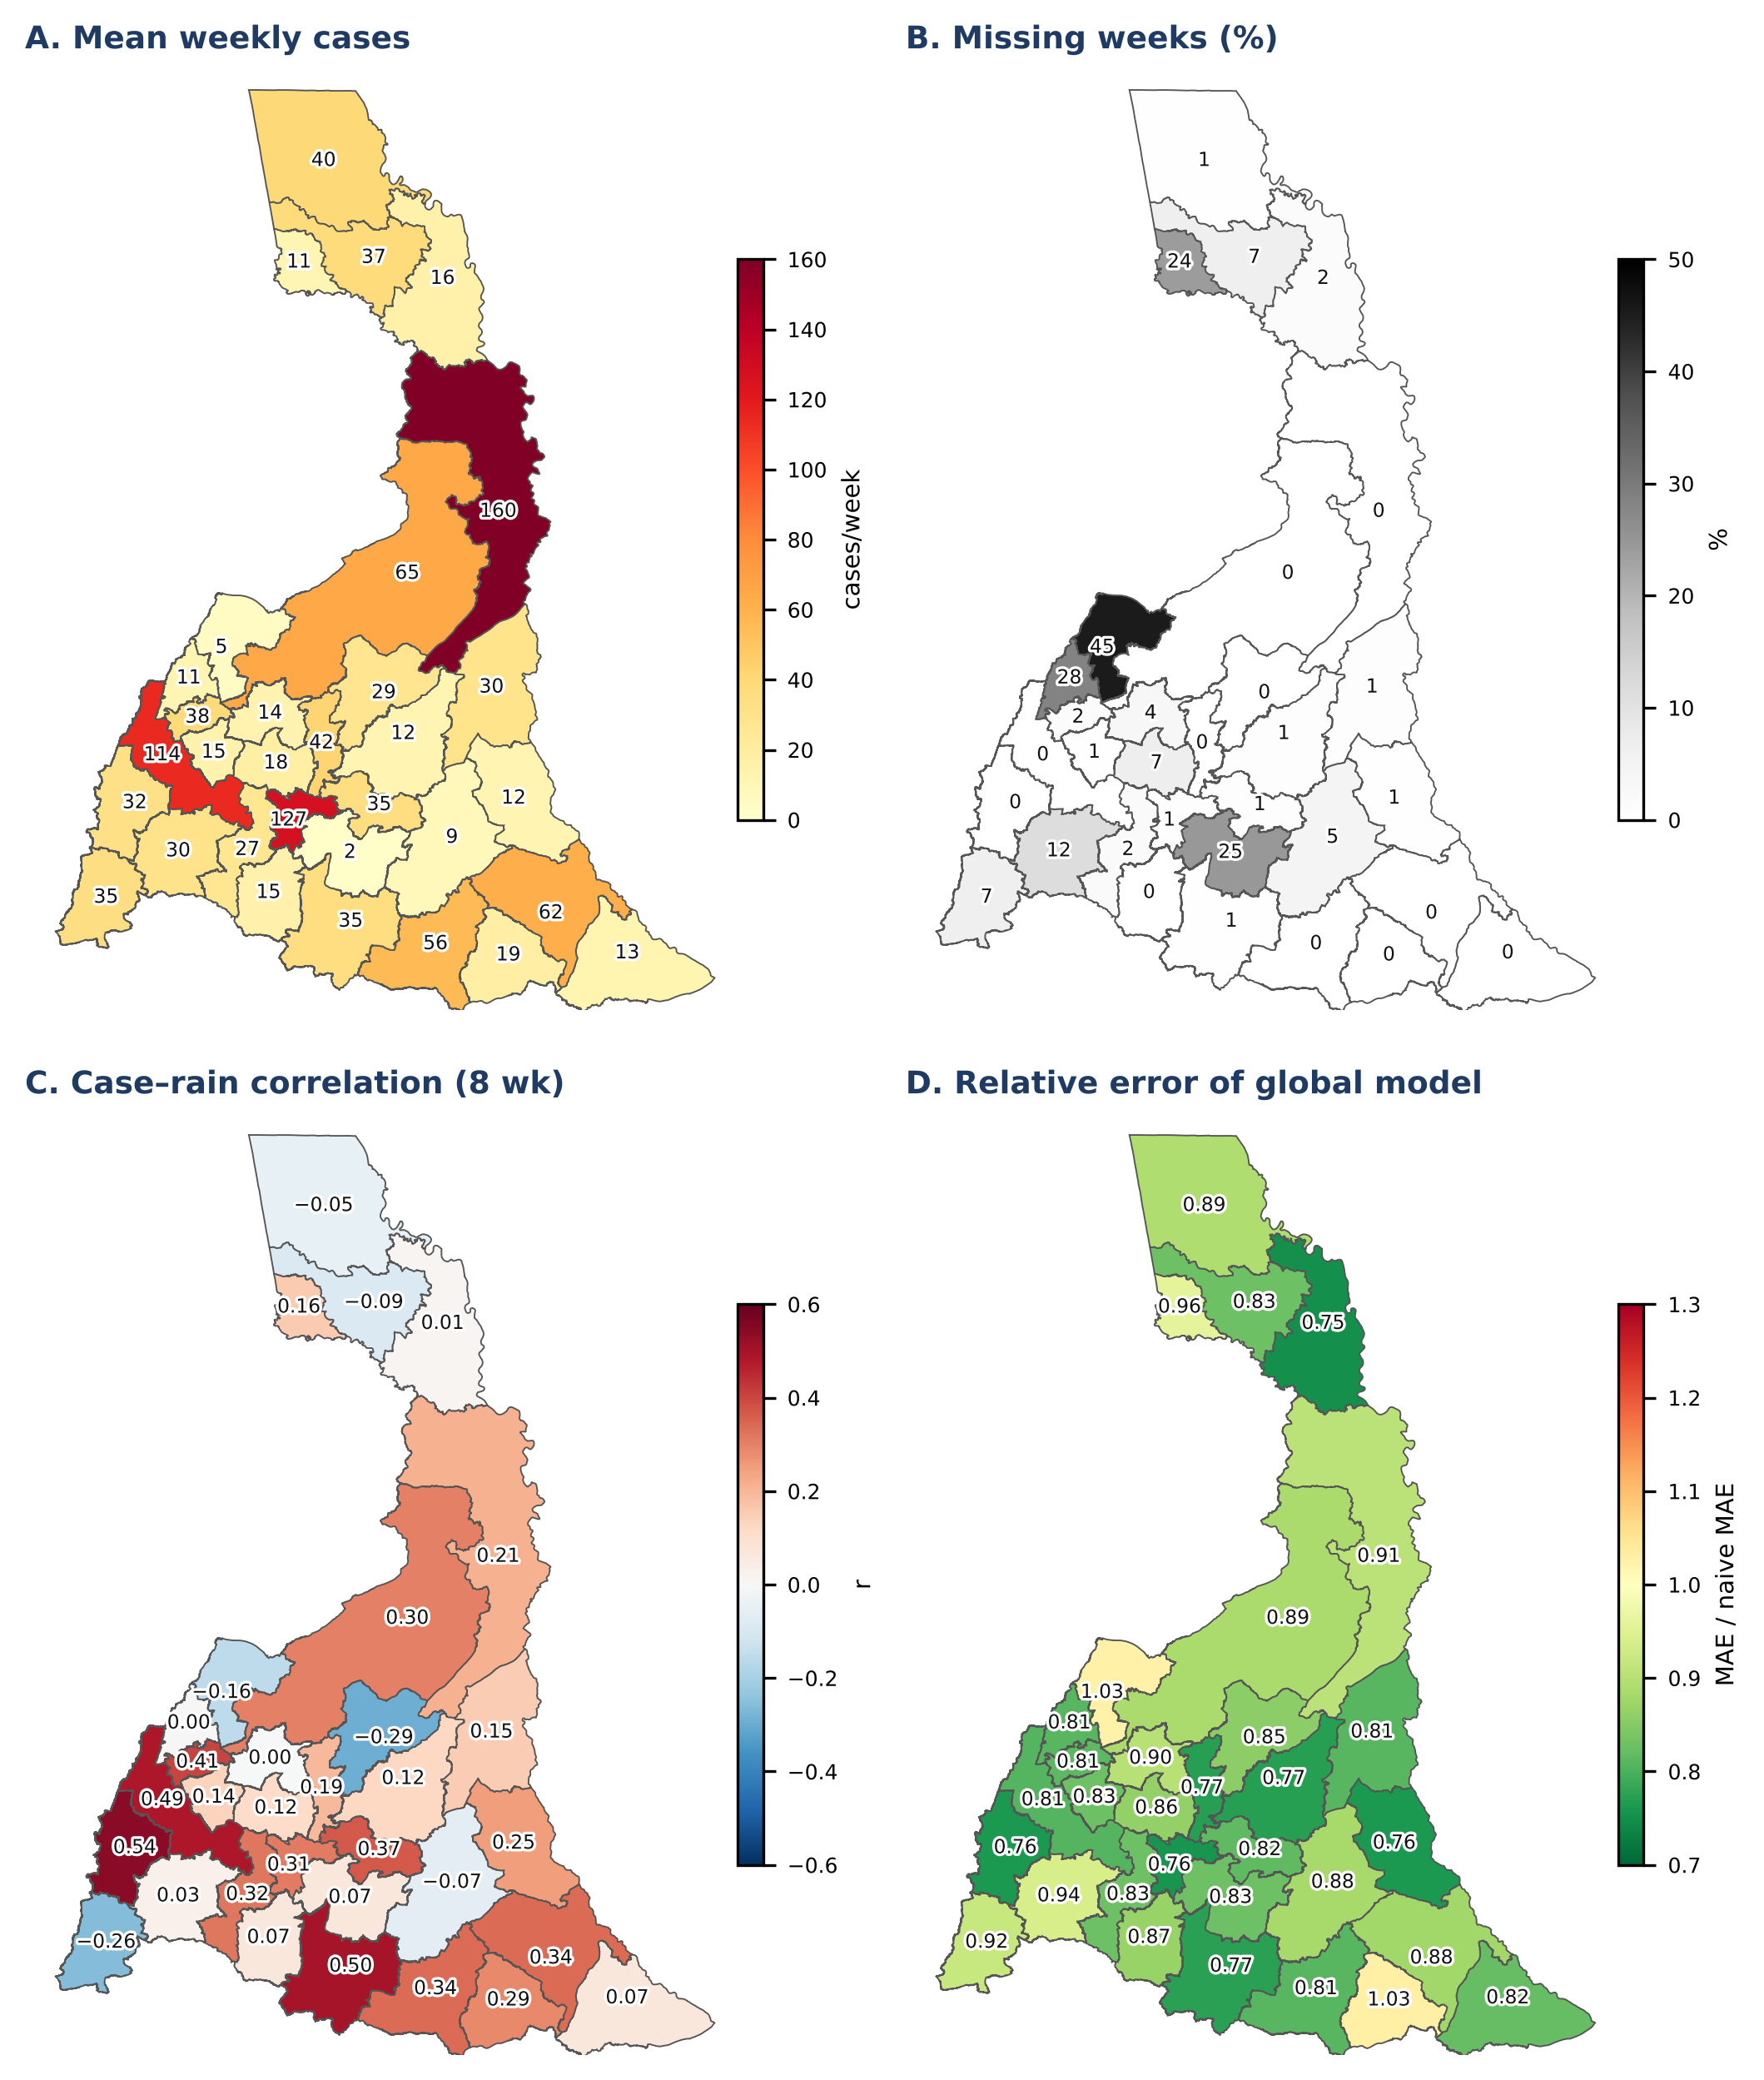
\includegraphics[width=0.92\linewidth]{figures/en_cartes_composite.png}\caption{Results by health district: (A) mean weekly cases; (B) proportion of missing weeks; (C) correlation between cases and rainfall at an 8-week lag; (D) error of the global model relative to the naive method at four weeks (below 1: better). District names are shown in Figure~\ref{fig:f2a_reference} and detailed values in Appendix A.}\label{fig:cartes}\end{figure}

\subsection{Data quality and series structure}
Missing data were concentrated at the start of the period (20.3\% of district-weeks in 2019, less than 1.2\% from 2022) and in four districts, several affected by insecurity: Kolofata (45.5\%), Mozogo (28.5\%), Mindif (24.7\%) and Fotokol (24.1\%) (Figures~\ref{fig:cartes}B and~\ref{fig:f4_manquants}). The 417 flagged unusual values were spread throughout the year. Taylor's law gave an exponent of 1.37: variability increases faster than the level of cases, which justifies the log scale of the global model.

\fig{f4_manquants}{0.92}{Structure of missing weeks by district (rows, sorted by decreasing proportion) and by week (columns).}

Decomposition of the regional series showed an increasing trend until 2022, linked to network expansion, and a regular annual season with a peak every year between September and November (Figure~\ref{fig:f5_stl}); trend strength was 0.77 and seasonal strength 0.57. The series was non-stationary in level but became stationary after week-to-week differencing (Table~\ref{tab:stat}). Cases in a given week were strongly related to those of previous weeks, with a rise around 52 weeks reflecting annual seasonality (Figure~\ref{fig:f7_acf}; Ljung–Box, $p<0.001$). The ARIMA(2,1,1) model left uncorrelated residuals ($p=0.71$ at 4 weeks). These results guided model choice: forecasting the change in cases rather than their level, and accounting for time of year.

\fig{f5_stl}{0.9}{Decomposition of the weekly regional series into trend, season and remainder (STL, 52-week period).}

\begin{table}[!htbp]\centering\small
\caption{Stationarity tests of the weekly regional series, 2019–2025.}\label{tab:stat}
\begin{tabularx}{\linewidth}{@{}L rrrr L@{}}\toprule
Transformation & ADF & $p$ (ADF) & KPSS & $p$ (KPSS) & Conclusion \\\midrule
Level & $-3.22$ & 0.019 & 2.13 & $<0.01$ & Non-stationary (trend) \\
Logarithm & $-3.21$ & 0.019 & 2.09 & $<0.01$ & Non-stationary (trend) \\
First difference & $-26.11$ & $<0.001$ & 0.06 & $>0.10$ & Stationary \\
Seasonal difference (52) & $-4.43$ & $<0.001$ & 0.37 & 0.09 & Stationary \\\bottomrule
\end{tabularx}
\par\smallskip\footnotesize\raggedright ADF: the null hypothesis is non-stationarity; KPSS: the null hypothesis is stationarity.
\end{table}

\fig{f7_acf}{0.9}{Autocorrelation (ACF) and partial autocorrelation (PACF) of the regional series, in level and after differencing. The grey band shows the 95\% confidence interval.}

\subsection{Rainfall sets the timing of the season}
The typhoid season consistently followed the rainy season (Figure~\ref{fig:f6_indices}). June to September accounted for 88\% of rainfall, peaking in August. Relative to trend, cases were lowest in June (16\% below normal) and highest in October (24\% above), about two months after the rainfall peak. The correlation between detrended cases and previous rainfall increased with the lag and peaked at 0.54 for 8 weeks (Figure~\ref{fig:f8_correlation}), as predicted by the model.

\fig{f6_indices}{0.85}{Monthly seasonal indices of typhoid cases (line; 1 = mean level of the year) and monthly distribution of rainfall (bars), Far North Region, 2019–2025.}

\fig{f8_correlation}{0.88}{Correlation between detrended weekly cases and rainfall accumulated over the previous 4 weeks (blue) or its anomaly relative to normal (orange), by lag in weeks. The grey band shows the 5\% significance threshold.}

The link was clear (correlation of at least 0.30) in 10 districts, mainly in the south-west and centre of the region: Mogode (0.54), Kaele (0.50), Mokolo (0.49), Koza (0.41), Maroua 3 (0.37), Guidiguis (0.34), Yagoua (0.34), Gazawa (0.32), Maroua 1 (0.31) and Mora (0.30) (Figure~\ref{fig:cartes}C). It was stronger in districts reporting more cases ($\rho=0.49$; $p=0.004$) and with more complete data ($\rho=-0.48$; $p=0.005$).

\subsection{Rainfall does not set the intensity of peaks}
A wetter-than-normal season did not lead to more cases: the correlation with rainfall anomalies was even slightly negative ($r=-0.19$ at 8 weeks; Figure~\ref{fig:f8_correlation}), and no district showed a notable positive association. In 2023, one of the driest years (623 mm), one of the most marked peaks of the period was observed (Table~\ref{tab:fac}, Figure~\ref{fig:f3_serie}).

\subsection{Regional forecasts}
At regional level, no method forecast significantly better than the naive method at one or four weeks (Table~\ref{tab:reg}). Adding rainfall, temperature and humidity did not improve XGBoost accuracy ($p=0.31$ at one week; $p=0.77$ at four weeks). All models followed the peaks with a delay (Figure~\ref{fig:f10_previsions}).

\begin{table}[!htbp]\centering\small
\caption{Accuracy of regional forecasts, 2023–2025 (156 weeks at one week, 153 at four weeks). MAE and RMSE in cases per week.}\label{tab:reg}
\begin{tabular}{@{}llrrrrl@{}}\toprule
Horizon & Method & MAE & RMSE & MAPE (\%) & Gain vs naive (\%) & $p$ \\\midrule
\multirow{6}{*}{1 week} & ARIMA & 102.3 & 127.5 & 7.6 & +4.7 & 0.15 \\
 & XGBoost & 105.4 & 135.8 & 7.7 & +1.8 & 0.68 \\
 & Naive (benchmark) & 107.3 & 135.2 & 7.9 & -- & -- \\
 & XGBoost with climate & 108.5 & 141.2 & 7.9 & $-1.1$ & 0.80 \\
 & Prophet & 132.3 & 174.9 & 9.4 & $-23.3$ & 0.013\,$^{\dagger}$ \\
 & Same week last year & 208.9 & 271.0 & 14.8 & $-94.7$ & $<0.001$\,$^{\dagger}$ \\\midrule
\multirow{6}{*}{4 weeks} & XGBoost with climate & 142.4 & 192.5 & 10.3 & +10.7 & 0.15 \\
 & XGBoost & 143.9 & 189.7 & 10.3 & +9.8 & 0.22 \\
 & Prophet & 145.5 & 195.2 & 10.2 & +8.8 & 0.48 \\
 & ARIMA & 153.8 & 203.0 & 11.1 & +3.6 & 0.41 \\
 & Naive (benchmark) & 159.5 & 211.9 & 11.6 & -- & -- \\
 & Same week last year & 210.9 & 273.1 & 14.9 & $-32.2$ & 0.06 \\\bottomrule
\end{tabular}
\par\smallskip\footnotesize\raggedright Diebold–Mariano test. $^{\dagger}$ Significantly less accurate than the naive method.
\end{table}

\fig{f10_previsions}{0.95}{Four-week-ahead regional forecasts, 2023–2025: observed cases and forecasts of the main methods.}

\subsection{District forecasts}
At district level, the global model was the most accurate (Table~\ref{tab:dist}, Figure~\ref{fig:f11_districts}). Across districts, it reduced error by 13\% at one week and 15\% at four weeks relative to the naive method ($p<0.001$), and by 2–5\% relative to ARIMA ($p=0.001$ and 0.005). It was significantly less accurate than the naive method in no district; only Kar Hay and Kolofata were not better forecast (Figure~\ref{fig:cartes}D). District-specific models, lacking sufficient data, did hardly better than the naive method.

\begin{table}[!htbp]\centering\small
\caption{Accuracy of district forecasts, 32 districts, 2023–2025.}\label{tab:dist}
\begin{tabularx}{\linewidth}{@{}l >{\raggedright\arraybackslash}p{3.6cm} R R R@{}}\toprule
Horizon & Method & Median relative error (naive = 1) & Districts better forecast than naive & Significantly better / worse \\\midrule
\multirow{4}{*}{1 week} & Global model & 0.87 & 31 & 27 / 0 \\
 & ARIMA by district & 0.88 & 30 & 17 / 1 \\
 & XGBoost by district & 0.98 & 21 & 2 / 1 \\
 & Same week last year & 1.44 & 1 & 0 / 29 \\\midrule
\multirow{4}{*}{4 weeks} & Global model & 0.83 & 30 & 21 / 0 \\
 & ARIMA by district & 0.89 & 30 & 16 / 1 \\
 & XGBoost by district & 0.96 & 18 & 4 / 0 \\
 & Same week last year & 1.24 & 3 & 0 / 14 \\\bottomrule
\end{tabularx}
\end{table}

\fig{f11_districts}{0.82}{Error relative to the naive method, by district and method, at four weeks. Districts are sorted by global model error; a value below 1 indicates a gain.}

To forecast, the global model relied mainly on current-week cases (19.5\% of importance), the 13-week mean (12.1\%), previous-week cases and the district's usual level (11.1\% each); time of year and the same week of the previous year together accounted for 21.4\% (Figure~\ref{fig:f12_importance}).

\fig{f12_importance}{0.82}{Relative importance of predictors in the global model for four-week-ahead forecasts.}

\subsection{Sensitivity analyses}
Regional conclusions were unchanged after excluding districts with incomplete data (Table~\ref{tab:sens}). The rainfall–case lag was identical in all scenarios. The XGBoost gain was larger with only complete-data districts and then became borderline significant; given the number of comparisons, this result should be interpreted with caution.

\begin{table}[!htbp]\centering\small
\caption{Sensitivity analyses: four-week regional forecasts by districts included.}\label{tab:sens}
\begin{tabularx}{\linewidth}{@{}L r r r r r r@{}}\toprule
Districts included & $n$ & XGBoost (\%) & $p$ & With climate (\%) & ARIMA (\%) & Rain $r$ \\\midrule
All & 32 & +9.8 & 0.22 & +10.7 & +3.6 & 0.42 \\
Less than 20\% missing weeks & 28 & +8.8 & 0.27 & +10.5 & +3.4 & 0.42 \\
Less than 5\% missing weeks & 24 & +16.4 & 0.053 & +16.2 & $-0.6$ & 0.47 \\
No missing weeks & 9 & +12.3 & 0.044 & +15.2 & +4.3 & 0.43 \\\bottomrule
\end{tabularx}
\par\smallskip\footnotesize\raggedright Gains are reductions in MAE relative to the naive method; $r$: rainfall–case correlation at 8 weeks, on raw series.
\end{table}

\section{Discussion}
In the Far North Region of Cameroon, rainfall sets the timing of the typhoid season but not its intensity. Cases peak every year in October, about two months after the rainfall peak, whereas a wetter-than-normal season does not lead to more cases and rainfall does not improve short-term forecasts.

\subsection{What the mathematical model explains}
These two findings match the two predictions of the transmission model. The two-month lag is consistent with the chain described by equation~\eqref{eq:pluie}: progressive contamination of wells and ponds during the rainy season, incubation, then consultation and reporting. In Nepal, cases also follow the monsoon, with a lag of about one month after floods [\hyperlink{ref9}{9}]; the longer lag observed here may reflect the context of the Far North, where water sources become progressively contaminated [\hyperlink{ref27}{27}]. The saturating force of infection~\eqref{eq:lambda} offers an explanation for the absence of an effect of rainfall intensity: during the rainy season, the environment may already be contaminated enough for extra rainfall to hardly change risk. Peak intensity would then depend on other factors, such as access to safe water, sanitation, population movements or diagnostic practices. This explanation remains a hypothesis that water quality measurements could test.

This mechanism also explains why rainfall does not improve forecasts: if its information reduces to the timing of the season, it is already contained in recent cases and the time of year. This finding does not contradict the Nepalese study, where floods explained part of the variation in cases [\hyperlink{ref9}{9}]: explaining variation, seasonality included, is not the same as improving a forecast that already knows the season.

\subsection{Forecasting at district level}
The global model succeeds where district-specific models fail because it learns common patterns across all districts, such as the shape of the season or the persistence of cases, while accounting for each district's own level. This is consistent with the forecasting literature [\hyperlink{ref21}{21},\hyperlink{ref22}{22}] and with Dixon et al., who trained a single model on regions of seven countries [\hyperlink{ref8}{8}]. At regional level, however, no method beats the naive benchmark: the regional series is too smooth for a complex model to bring a measurable gain. Shashvat et al. concluded that exponential smoothing was superior for typhoid in Chandigarh over 48 months, without a statistical test [\hyperlink{ref7}{7}]; our results are a reminder that models should always be compared with a simple benchmark, using a formal test [\hyperlink{ref10}{10}].

\subsection{Reading DHIS2 trends with caution}
The rise in reported cases between 2019 and 2022 mainly reflects the expansion of the surveillance network: the number of reporting facilities tripled while cases increased by 72\%, and the increase has been only 20\% since the network stabilised. Any reading of DHIS2 trends should account for reporting completeness.

\subsection{Implications for decision-makers}
The findings translate into concrete actions (Table~\ref{tab:actions}).

\begin{table}[!htbp]\centering\small
\caption{Operational recommendations from the study.}\label{tab:actions}
\begin{tabularx}{\linewidth}{@{}>{\raggedright\arraybackslash}p{4.3cm} L@{}}\toprule
When / where & Recommended action \\\midrule
June–July & Pre-position supplies (antibiotics, tests, fluids) and launch water, hygiene and chlorination messages, before the October peak. \\
August–November & Strengthen vigilance and weekly monitoring; the peak occurs about two months after maximum rainfall. \\
Mogode, Kaele, Mokolo, Koza, Maroua 1 and 3, Guidiguis, Yagoua, Gazawa, Mora & Prioritise seasonal preparedness: the link with rainfall is strongest. \\
Kolofata, Mozogo, Mindif, Fotokol & First strengthen reporting regularity: more than 20\% missing weeks. \\
Whole region & Use a global model, retrained weekly, alongside DHIS2 alert thresholds; invest in water, sanitation and diagnostic confirmation to reduce peak intensity. \\\bottomrule
\end{tabularx}
\end{table}

\subsection{Strengths and limitations}
The study covers all districts of a region over seven years, with documented pre-processing and a strict three-year evaluation protocol. Three limitations should be noted.

\begin{enumerate}[label=\arabic*.,leftmargin=1.6em]
\item \textbf{Widal diagnosis and malaria co-endemicity.} Reported cases mainly rely on the Widal serological test, whose specificity is low in endemic areas [\hyperlink{ref3}{3}]; cross-reactions are possible, notably with malaria, whose seasonal peak coincides with the end of the rainy season. This bias may amplify the apparent magnitude of the October peak. However, as diagnostic practices remained constant over 2019–2025, it does not undermine the analysis of seasonal timing or the relative comparison of forecasting methods.
\item \textbf{Missing data.} Four districts affected by insecurity (Kolofata, Mozogo, Mindif, Fotokol) have more than 20\% missing weeks, and imputation may have smoothed real variation; evaluation on observed weeks only and sensitivity analyses limit this effect.
\item \textbf{Lack of weekly cofactors.} Access to water, sanitation and population movements, likely to drive peak intensity, were not available at weekly resolution.
\end{enumerate}

\section{Conclusion}
In the Far North Region of Cameroon, rainfall tells \textit{when} the typhoid season will come, about two months ahead, but not \textit{how many} cases it will produce. Districts can therefore plan their preparedness from July, while reducing peaks depends on access to safe water, sanitation and diagnosis. For short-term operational forecasting, a single model shared across districts, fed with routine DHIS2 data, provides a simple and validated baseline.

\section*{Declarations}
\small
\textbf{Supplementary material.} S1: full mathematical formulation (pre-processing, exploratory analysis, transmission model, forecasting models and statistical tests).
\textbf{Author contributions (CRediT taxonomy).} Kazoune Bouba Israel: conceptualisation, methodology, software, data curation, formal analysis, visualisation, writing -- original draft. Maïrousgou Céline: resources, data curation, validation, writing -- review and editing. Kidwang Jean Pierre: validation, writing -- review and editing. Kolaye Guilsou Gabriel (study supervisor): conceptualisation, methodology, supervision, validation, project administration, writing -- review and editing. All authors read and approved the final manuscript.
\textbf{Funding.} This research received no external funding.
\textbf{Ethics.} The study uses only aggregated routine surveillance data, without individual information; their use was authorised by the Regional Delegation of Public Health of the Far North (DRSP-EN).
\textbf{Data and code availability.} District-level aggregated cases are available from the authors subject to approval by the Ministry of Public Health; climate data are public (NASA POWER); analysis scripts are deposited in the public GitHub repository \url{https://github.com/israel-12/typhoide-extreme-nord}.
\textbf{Acknowledgements.} To the staff of the Regional Delegation and of health facilities who report surveillance data every week.
\textbf{Competing interests.} None.

\section*{References}
\footnotesize
\noindent\textit{Reference numbers in the text and DOIs are clickable links.}
\begin{enumerate}[label={[\arabic*]},leftmargin=2.2em,itemsep=0.5pt]
\item\hypertarget{ref1}{}Stanaway JD, et al. The global burden of typhoid and paratyphoid fevers: a systematic analysis for the Global Burden of Disease Study 2017. \textit{Lancet Infect Dis.} 2019;19:369--381. \href{https://doi.org/10.1016/S1473-3099(18)30685-6}{\nolinkurl{doi:10.1016/S1473-3099(18)30685-6}}
\item\hypertarget{ref2}{}Antillón M, Warren JL, Crawford FW, Weinberger DM, Kürüm E, Pak GD, Marks F, Pitzer VE. The burden of typhoid fever in low- and middle-income countries: a meta-regression approach. \textit{PLoS Negl Trop Dis.} 2017;11(2):e0005376. \href{https://doi.org/10.1371/journal.pntd.0005376}{\nolinkurl{doi:10.1371/journal.pntd.0005376}}
\item\hypertarget{ref3}{}Yemeli Piankeu J, et al. Epidemiology and performances of Typhidot immunoassay and Widal slide agglutination in the diagnosis of typhoid fever in febrile patients in Bafoussam City, Cameroon. \textit{Can J Infect Dis Med Microbiol.} 2024;2024:6635067. \href{https://doi.org/10.1155/2024/6635067}{\nolinkurl{doi:10.1155/2024/6635067}}
\item\hypertarget{ref4}{}Ministère de la Santé publique du Cameroun (MINSANTE). \textit{Plan opérationnel de mise en œuvre du DHIS2 2022--2024.} Yaoundé : MINSANTE ; 2022.
\item\hypertarget{ref5}{}Tilahun GT, Makinde OD, Malonza D. Modelling and optimal control of typhoid fever disease with cost-effective strategies. \textit{Comput Math Methods Med.} 2017;2017:2324518. \href{https://doi.org/10.1155/2017/2324518}{\nolinkurl{doi:10.1155/2017/2324518}}
\item\hypertarget{ref6}{}Sabir Z, Abdelkawy MA, Mehmood MA, Bayram M. Modeling typhoid dynamics using recurrent neural networks with Bayesian regularization. \textit{Comput Biol Chem.} 2026. \href{https://doi.org/10.1016/j.compbiolchem.2025.108790}{\nolinkurl{doi:10.1016/j.compbiolchem.2025.108790}}
\item\hypertarget{ref7}{}Shashvat K, Basu R, Bhondekar AP, Lamba S, Verma K, Kaur A. Comparison of time series models predicting trends in typhoid cases in northern India. \textit{Southeast Asian J Trop Med Public Health.} 2019;50:347--356.
\item\hypertarget{ref8}{}Dixon S, Keshavamurthy R, Farber DH, Stevens A, Pazdernik KT, Charles LE. A comparison of infectious disease forecasting methods across locations, diseases, and time. \textit{Pathogens.} 2022;11:185. \href{https://doi.org/10.3390/pathogens11020185}{\nolinkurl{doi:10.3390/pathogens11020185}}
\item\hypertarget{ref9}{}Baral K, Bista R, Kaasbøll J. Predictive modeling of typhoid incidence in Nepal under extreme climate change scenarios using machine learning algorithm. In: \textit{ICT4D 2026}, IFIP AICT 784. Springer; 2026. p.~216--237.
\item\hypertarget{ref10}{}Makridakis S, Spiliotis E, Assimakopoulos V. Statistical and machine learning forecasting methods: concerns and ways forward. \textit{PLoS ONE.} 2018;13:e0194889. \href{https://doi.org/10.1371/journal.pone.0194889}{\nolinkurl{doi:10.1371/journal.pone.0194889}}
\item\hypertarget{ref11}{}NASA Langley Research Center. POWER (Prediction Of Worldwide Energy Resources) Project: daily meteorological data. \url{https://power.larc.nasa.gov}
\item\hypertarget{ref12}{}Hampel FR. The influence curve and its role in robust estimation. \textit{J Am Stat Assoc.} 1974;69:383--393. \href{https://doi.org/10.1080/01621459.1974.10482962}{\nolinkurl{doi:10.1080/01621459.1974.10482962}}
\item\hypertarget{ref13}{}Taylor LR. Aggregation, variance and the mean. \textit{Nature.} 1961;189:732--735. \href{https://doi.org/10.1038/189732a0}{\nolinkurl{doi:10.1038/189732a0}}
\item\hypertarget{ref14}{}Cleveland RB, Cleveland WS, McRae JE, Terpenning I. STL: a seasonal-trend decomposition procedure based on loess. \textit{J Off Stat.} 1990;6:3--73.
\item\hypertarget{ref15}{}Dickey DA, Fuller WA. Distribution of the estimators for autoregressive time series with a unit root. \textit{J Am Stat Assoc.} 1979;74:427--431. \href{https://doi.org/10.1080/01621459.1979.10482531}{\nolinkurl{doi:10.1080/01621459.1979.10482531}}
\item\hypertarget{ref16}{}Kwiatkowski D, Phillips PCB, Schmidt P, Shin Y. Testing the null hypothesis of stationarity against the alternative of a unit root. \textit{J Econom.} 1992;54:159--178. \href{https://doi.org/10.1016/0304-4076(92)90104-Y}{\nolinkurl{doi:10.1016/0304-4076(92)90104-Y}}
\item\hypertarget{ref17}{}Ljung GM, Box GEP. On a measure of lack of fit in time series models. \textit{Biometrika.} 1978;65:297--303. \href{https://doi.org/10.1093/biomet/65.2.297}{\nolinkurl{doi:10.1093/biomet/65.2.297}}
\item\hypertarget{ref18}{}Box GEP, Jenkins GM, Reinsel GC, Ljung GM. \textit{Time Series Analysis: Forecasting and Control.} 5th ed. Wiley; 2015.
\item\hypertarget{ref19}{}Taylor SJ, Letham B. Forecasting at scale. \textit{Am Stat.} 2018;72:37--45. \href{https://doi.org/10.1080/00031305.2017.1380080}{\nolinkurl{doi:10.1080/00031305.2017.1380080}}
\item\hypertarget{ref20}{}Chen T, Guestrin C. XGBoost: a scalable tree boosting system. In: \textit{Proc. 22nd ACM SIGKDD.} 2016. p.~785--794. \href{https://doi.org/10.1145/2939672.2939785}{\nolinkurl{doi:10.1145/2939672.2939785}}
\item\hypertarget{ref21}{}Montero-Manso P, Hyndman RJ. Principles and algorithms for forecasting groups of time series: locality and globality. \textit{Int J Forecast.} 2021;37:1632--1653. \href{https://doi.org/10.1016/j.ijforecast.2021.03.004}{\nolinkurl{doi:10.1016/j.ijforecast.2021.03.004}}
\item\hypertarget{ref22}{}Makridakis S, Spiliotis E, Assimakopoulos V. M5 accuracy competition: results, findings, and conclusions. \textit{Int J Forecast.} 2022;38:1346--1364. \href{https://doi.org/10.1016/j.ijforecast.2021.11.013}{\nolinkurl{doi:10.1016/j.ijforecast.2021.11.013}}
\item\hypertarget{ref23}{}Hyndman RJ, Athanasopoulos G. \textit{Forecasting: Principles and Practice.} 3rd ed. OTexts; 2021. \url{https://otexts.com/fpp3/}
\item\hypertarget{ref24}{}Willmott CJ, Matsuura K. Advantages of the mean absolute error (MAE) over the root mean square error (RMSE) in assessing average model performance. \textit{Clim Res.} 2005;30:79--82. \href{https://doi.org/10.3354/cr030079}{\nolinkurl{doi:10.3354/cr030079}}
\item\hypertarget{ref25}{}Diebold FX, Mariano RS. Comparing predictive accuracy. \textit{J Bus Econ Stat.} 1995;13:253--263. \href{https://doi.org/10.1080/07350015.1995.10524599}{\nolinkurl{doi:10.1080/07350015.1995.10524599}}
\item\hypertarget{ref26}{}Harvey D, Leybourne S, Newbold P. Testing the equality of prediction mean squared errors. \textit{Int J Forecast.} 1997;13:281--291. \href{https://doi.org/10.1016/S0169-2070(96)00719-4}{\nolinkurl{doi:10.1016/S0169-2070(96)00719-4}}
\item\hypertarget{ref27}{}Saad NJ, Lynch VD, Antillón M, Yang C, Crump JA, Pitzer VE. Seasonal dynamics of typhoid and paratyphoid fever. \textit{Sci Rep.} 2018;8:6870. \href{https://doi.org/10.1038/s41598-018-25234-w}{\nolinkurl{doi:10.1038/s41598-018-25234-w}}
\end{enumerate}

\normalsize
\section*{Appendix A. Results by health district}
\begin{table}[!htbp]\centering\scriptsize\setlength{\tabcolsep}{4pt}
\caption{Characteristics and results by health district, sorted by total cases (relative MAE of the global model versus the naive model).}\label{tab:annexe}
\begin{tabular}{@{}lrrrrrrl@{}}\toprule
District & Total cases & Cases/week & Missing (\%) & Rain $r$ (8 wk) & Rel. MAE ($h$=1) & Rel. MAE ($h$=4) & Best model ($h$=4) \\\midrule
Kousseri & 58,276 & 159.7 & 0.0 & 0.21 & 1.00 & 0.91 & ARIMA \\
Maroua 1 & 46,073 & 127.3 & 0.8 & 0.31 & 0.92 & 0.76 & Global XGBoost \\
Mokolo & 41,745 & 114.4 & 0.0 & 0.49 & 0.88 & 0.81 & Global XGBoost \\
Mora & 23,816 & 65.2 & 0.0 & 0.30 & 0.93 & 0.89 & ARIMA \\
Yagoua & 22,763 & 62.4 & 0.0 & 0.34 & 0.89 & 0.88 & Global XGBoost \\
Guidiguis & 20,483 & 56.1 & 0.0 & 0.34 & 0.87 & 0.81 & Global XGBoost \\
Maroua 2 & 15,396 & 42.2 & 0.0 & 0.19 & 0.88 & 0.77 & Global XGBoost \\
Mada & 14,366 & 39.6 & 0.5 & $-$0.05 & 0.89 & 0.89 & ARIMA \\
Koza & 13,692 & 38.1 & 1.6 & 0.41 & 0.89 & 0.81 & Global XGBoost \\
Kaele & 12,757 & 35.1 & 0.5 & 0.50 & 0.84 & 0.77 & Global XGBoost \\
Maroua 3 & 12,664 & 35.1 & 1.1 & 0.37 & 0.85 & 0.82 & Global XGBoost \\
Makary & 12,579 & 36.9 & 6.6 & $-$0.09 & 0.84 & 0.83 & ARIMA \\
Bourha & 11,862 & 34.8 & 6.6 & $-$0.26 & 0.82 & 0.92 & ARIMA \\
Mogode & 11,851 & 32.5 & 0.0 & 0.54 & 0.88 & 0.76 & Global XGBoost \\
Maga & 10,777 & 29.9 & 1.1 & 0.15 & 0.84 & 0.81 & Global XGBoost \\
Pette & 10,492 & 28.7 & 0.0 & $-$0.29 & 0.86 & 0.85 & Global XGBoost \\
Hina & 9,729 & 30.1 & 11.5 & 0.03 & 0.94 & 0.94 & ARIMA \\
Gazawa & 9,681 & 27.1 & 2.2 & 0.32 & 0.81 & 0.83 & Global XGBoost \\
Kar Hay & 6,908 & 19.0 & 0.3 & 0.29 & 0.95 & 1.03 & ARIMA \\
Meri & 6,045 & 17.8 & 6.8 & 0.12 & 0.87 & 0.86 & Global XGBoost \\
Goulfey & 5,678 & 15.9 & 1.9 & 0.01 & 0.72 & 0.75 & Global XGBoost \\
Moutourwa & 5,608 & 15.4 & 0.3 & 0.07 & 0.83 & 0.87 & Global XGBoost \\
Roua & 5,416 & 14.9 & 0.5 & 0.14 & 0.86 & 0.83 & Global XGBoost \\
Tokombere & 4,834 & 13.7 & 3.6 & 0.00 & 0.84 & 0.90 & Global XGBoost \\
Guere & 4,757 & 13.0 & 0.0 & 0.07 & 0.86 & 0.82 & Global XGBoost \\
Bogo & 4,521 & 12.5 & 0.8 & 0.12 & 0.79 & 0.77 & ARIMA \\
Vele & 4,483 & 12.3 & 0.5 & 0.25 & 0.83 & 0.76 & Global XGBoost \\
Fotokol & 3,166 & 11.4 & 24.1 & 0.16 & 0.90 & 0.96 & ARIMA \\
Mozogo & 2,984 & 11.4 & 28.5 & 0.00 & 0.84 & 0.81 & Global XGBoost \\
Moulvoudaye & 2,959 & 8.5 & 4.7 & $-$0.07 & 0.89 & 0.88 & Global XGBoost \\
Kolofata & 941 & 4.7 & 45.5 & $-$0.16 & 0.96 & 1.03 & Naive \\
Mindif & 608 & 2.2 & 24.7 & 0.07 & 0.87 & 0.83 & ARIMA \\
\bottomrule\end{tabular}
\end{table}

\end{document}
